\documentclass[10pt,oneside]{mwbk}

% ustawienia kodowania pliku i języka
\usepackage[T1]{polski}
\usepackage[utf8]{inputenc}

\usepackage{indentfirst}
\usepackage{graphicx}


% czcionka Times
\usepackage{times}

% odstępy na 1.5 (pomimo, iż linespread jest na 1.3
\linespread{1.3}

% dzielenie wyrazów – większe odstępy, mniej dzielenia
\hyphenpenalty=5000
\tolerance=5000

%import z pliku csv
%\usepackage{csvsimple}

%strona tytułowa
\renewcommand {\maketitle}{
\begin {titlepage}
\begin {center}
	\LARGE
	\textbf {PROJEKTOWANIE ALGORYTMOW I METODY SZTUCZNEJ INTELIGENCJI}
	\newline
	\newline
	\textit {SPRAWOZDANIE Z  LABORATORIUM}
	\textbf{ Sortowanie quick poruwniane czasow sortowaia}
	\newline
	\begin{table}
	\begin{center}
	\begin{tabular}{rl}
	IMIĘ I NAZWISKO & Tomasz Piotrowski \\
	NR INDEKSU & 200524 \\	
	
	\end{tabular}

	\end{center}
	\end{table}
\end {center}
\end {titlepage}}

\renewcommand*\thesection{\arabic{section}} % zmiana numeracji sekcji 0.X -> X
\begin{document}
\maketitle
\section{Wstęp}
	
	\indent Quicksort w podstawowej wersji za piwot obiera środkowy element zbioru. Taki sposób jest często stosowany w implementacji algorytmu, jednak aby zminimalizować prawdopodobieństwo przypadku pesymistycznego można losowwo wybierać piwot. Dzięki czemu szansa na wystąpienie najgorszego przypadku są statystycznie znacznie mniejsze.\\
	\\
	\indent Celem tego ćwiczenia jest zSprawdzenie jaki wpływ na czas sortowania ma sposób doboru piwotu.
\newpage	
\section {Wyniki symulacji}

	\textbf{CZASY SORTOWANIA W PESYMISTYCZNYM PRZYPADKU}
	\\

	\begin{table}[!h]
	\centering
	\begin{tabular}{| l | l | l |}
	\hline
	Rozmiar & średnia z: & Czas         \\ \hline
1000&5&0\\ \hline
10000&5&0.0033\\ \hline
100000&5&0.04166\\ \hline
1000000&5&4.7833\\ \hline
10000000&5&53.94\\ \hline
	\end{tabular}
	\caption{Czas sortowania podstawowym Quicksortem}
	\end{table}
	
	
	\begin{table}[!h]
	\centering
	\begin{tabular}{| l | l | l |}
	\hline
		Rozmiar & średnia z: & Czas         \\ \hline
1000&5&0\\ \hline
10000&5&0.0027\\ \hline
100000&5&0.3001\\ \hline
1000000&5&3.876\\ \hline
10000000&5&42.65\\ \hline
	\end{tabular}
		\caption{Czas sortowania Quicksortem z losowym doborem piwotu}
	\end{table}
	
	
	\newpage
	\textbf{CZASY SORTOWANIA W ŚREDNIM PRZYPADKU}
	\\
	
	\begin{table}[!h]
	\centering
	\begin{tabular}{| l | l | l |}
	\hline
	Rozmiar & średnia z: & Czas         \\ \hline 
1000&5&0\\ \hline
10000&5&0.00396\\ \hline
100000&5&0.02\\ \hline
1000000&5&0.2666\\ \hline
10000000&5&3.0166\\ \hline
100000000&5&34.4567\\ \hline
	\end{tabular}
		\caption{Czas sortowania podstawowym Quicksortem}
	\end{table}
	

	\begin{table}[!h]
	\centering
	\begin{tabular}{| l | l | l |}
	\hline
		Rozmiar & średnia z: & Czas         \\ \hline
1000&5&0\\ \hline
10000&5&0.00333\\ \hline
100000&5&0.02\\ \hline
1000000&5&0.2133\\ \hline
10000000&5&2.4533\\ \hline
10000000&5&28.37\\ \hline
	\end{tabular}
	\caption{Czas sortowania Quicksortem z losowym doborem piwotu}
	\end{table}
\newpage
\section {Wykresy}
	\begin{figure}[!h]

	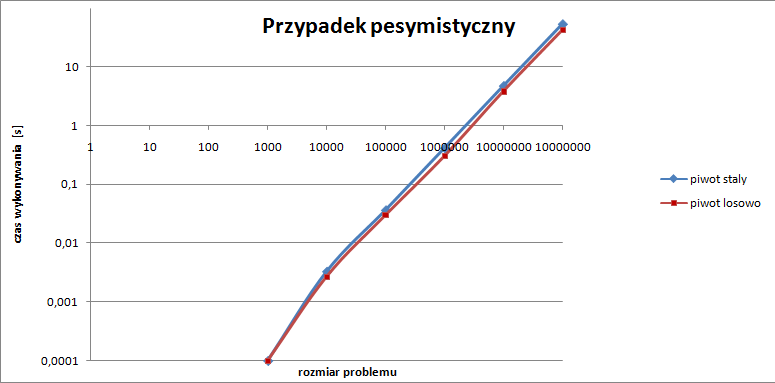
\includegraphics[scale=0.6]{rys/przypadek_pesymistyczny.png}
	\caption{ Złożoność obliczeniowa sortowania w przypadku pesymistycznym}

	\end{figure}
	
	\begin{figure}[!h]
	\centering
	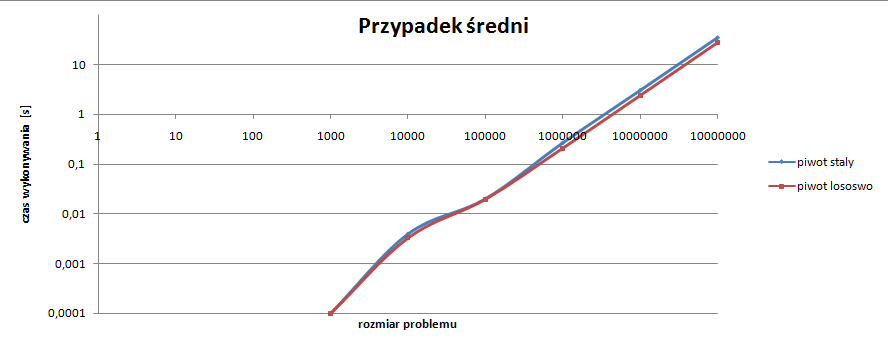
\includegraphics[scale=0.7]{rys/przypadek_sredni.png}
	\caption{ Złożoność obliczeniowa sortowania w przypadku srednim}
	\end{figure}
\newpage
\section {Wnioski}
\indent Po przeprowadzeniu symulacji zauważalna jest różnica w czasie wykonywania algorytmu dla obu metod
W obu przypadkach losowy dobór piwotu powoduje szybsze posortowanie zbioru niż w dobor stałego elementu zbioru.
\indent Zastosowanie tej metody wyboru piwotu usprawnia działanie sortowania szybkiego zmniejszając czas jego wykonywania. 
\end{document}